\section{Re-analysis under a common measurement boundary}
\label{sec:reanalysis}

Because the instrument differed across stacks, we report every result under three
energy definitions:

\begin{description}\itemsep2pt
  \item[as measured] CodeCarbon's total, instrument-confounded;
  \item[GPU only] the NVML energy counter alone --- the same instrument
        everywhere, and the only quantity attributable to the deep learning
        computation;
  \item[harmonised] GPU counter plus a single uniform \SI{107}{\watt} host model
        applied to every ecosystem.
\end{description}

\subsection{The rankings are not robust to the boundary}

\begin{table}[t]
\centering
\caption{Best and worst ecosystem, and spread, under each energy definition. The
identity of the worst ecosystem in training changes with the definition.}
\label{tab:spreads}
\small
\begin{tabular}{lllr}
\toprule
Phase & Energy definition & Best / Worst & Spread \\
\midrule
Training & as measured    & Rust/tch / Java/DL4J & \(4.58\times\) \\
Training & GPU only       & Rust/tch / R/torch   & \(8.54\times\) \\
Training & harmonised     & Rust/tch / R/torch   & \(9.94\times\) \\
Training & execution time & Rust/tch / R/torch   & \(11.63\times\) \\
\midrule
Inference & as measured    & C++/LibTorch / R/torch & \(7.28\times\) \\
Inference & GPU only       & C++/LibTorch / R/torch & \(9.30\times\) \\
Inference & harmonised     & C++/LibTorch / R/torch & \(8.83\times\) \\
Inference & execution time & C++/LibTorch / R/torch & \(8.47\times\) \\
\bottomrule
\end{tabular}
\end{table}

The headline figures quoted in the campaign --- \(4.6\times\) for training,
\(7.3\times\) for inference --- are the as-measured spreads. Under a common
boundary they become \(9.9\times\) and \(8.8\times\), and the worst ecosystem in
training changes identity.

\subsection{``Faster is not greener'' does not survive}

The campaign concludes that execution time is an unreliable proxy for energy. We
quantify the relationship rather than reading it off qualitative quadrants.

Within an ecosystem, energy is very nearly a deterministic linear function of
wall-clock time: the median \(R^2\) of energy on duration is \num{0.98}. This is
expected once Section~\ref{sec:instrument} is taken into account.

Across ecosystems, agreement between the energy ranking and the time ranking is:

\begin{center}
\small
\begin{tabular}{llrr}
\toprule
Phase & Energy definition & Spearman \(\rho\) & Discordant pairs \\
\midrule
Inference & as measured & 0.90 & 3 of 28 \\
Inference & GPU only    & 0.98 & 1 of 28 \\
Inference & harmonised  & \textbf{1.00} & \textbf{0 of 28} \\
\midrule
Training  & as measured & 0.95 & 2 of 28 \\
Training  & GPU only    & 0.93 & 2 of 28 \\
Training  & harmonised  & \textbf{0.98} & \textbf{1 of 28} \\
\bottomrule
\end{tabular}
\end{center}

Under a harmonised boundary the disagreement vanishes entirely for inference and
reduces to a single pair in training. The specific examples the manuscript gives
are exactly the pairs that disappear once the host power model is held constant.

\begin{figure}[t]
\centering
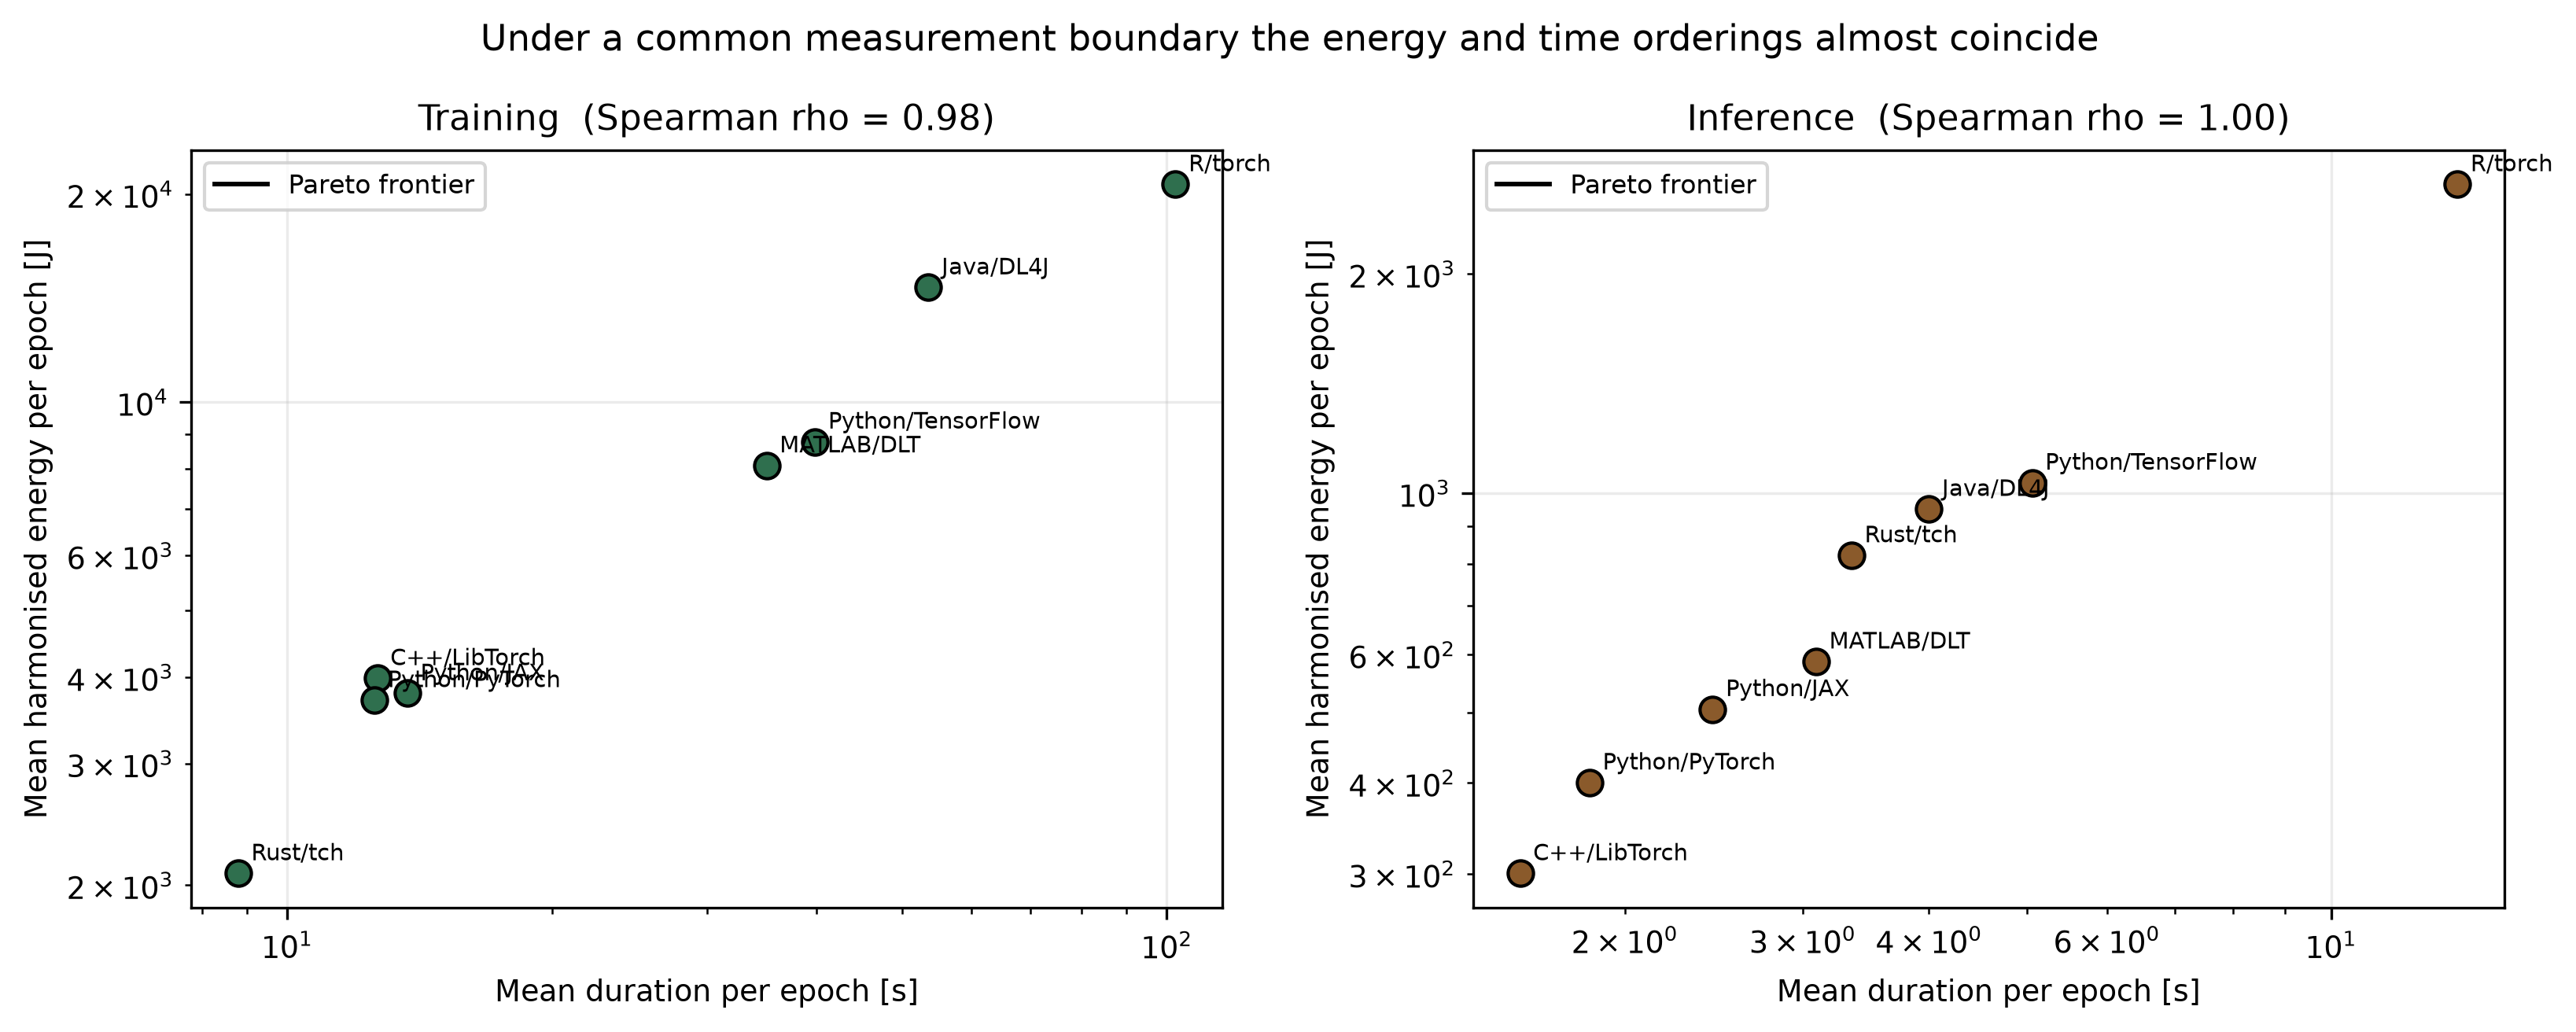
\includegraphics[width=\linewidth]{figures/fig_pareto.png}
\caption{Energy against duration per ecosystem under the harmonised boundary.
The orderings coincide for inference and differ by one pair in training; the
campaign's qualitative quadrant plot suggested a much weaker relationship.}
\label{fig:pareto}
\end{figure}

Decomposing energy as mean power times duration, \SI{98}{\percent} (inference) and
\SI{107}{\percent} (training) of the log spread is attributable to duration, with
a mean-power spread of only \(1.3\)--\(1.6\times\).

\subsection{The internal control group reproduces the whole effect}

Four of the eight ecosystems --- Python/PyTorch, C++/LibTorch, R/torch and
Rust/tch --- run the same LibTorch kernels. They are the study's natural control
group: any difference between them is binding, runtime and data-pipeline
overhead, not language.

Restricting the comparison to those four reproduces
\SIrange{98}{100}{\percent} of the full eight-stack spread on a log scale, in
every phase and under every energy definition. Whatever is being measured is
host-side.

We note that the group was not in fact controlled: the four stacks ran LibTorch
2.1.0, 2.5.x, 2.6.0 and 2.7.0 respectively --- six minor releases apart --- so
any difference between them also mixes in kernel, allocator and cuDNN changes.

\subsection{What the design can and cannot support}

Each of the 48 configurations was executed once, and the 30 epochs of a run are
repeated measurements of that run, sharing one initialisation, one JIT outcome,
one allocator state and one thermal trajectory. The effective number of
independent observations per configuration is one, not thirty.

We therefore report medians alongside means, bootstrap intervals over epochs
labelled explicitly as within-run dispersion, and effect sizes; and we do not
report a significance claim about ecosystems. Tests computed over epochs are
anti-conservative by an unknown factor: they compare the epochs of one run with
the epochs of another.

Separately, \num{158} rows (\SI{5.5}{\percent}) report a sampled GPU power of
\SI{0}{\watt} and \num{27} exceed the board limit, up to \SI{3054}{\watt}. These
are confined to CodeCarbon's \emph{sampled} power columns, which are unreliable
because \SI{69}{\percent} of the measured blocks are shorter than the
\SI{15}{\second} default sampling period. The energy columns come from the NVML
counter and show no such values.
